%%%%%%%
% Ch2 %
%%%%%%%

\chapter{Redresseur à diodes}
	
	Ils sont simples, bon marché et ne nécessitent aucun réglage, délivrent une tension continue essentiellement constante sur base d'une tension alternative. Il existe deux catégories de charges à alimenter, celles pour lesquelles il faut délivré une tension continue lisse et celle pour lesquelles il faut limiter la déformation du signal. Les équipements électroniques appartiennent à la 1ère catégorie, c'est pourquoi on retrouve un condensateur connecté entre les bornes de sortie qui permet de lisser le signal redressé. Les machines à courant continu, charges dites $RLE$, appartiennent à la 2è catégorie, nécessite un redresseur à thyristors (\textbf{commandable}) puisque celui à diode est \textbf{non-commandable}. La liste des symbole utilisé est repris ci-dessous.
	
	\begin{center}
	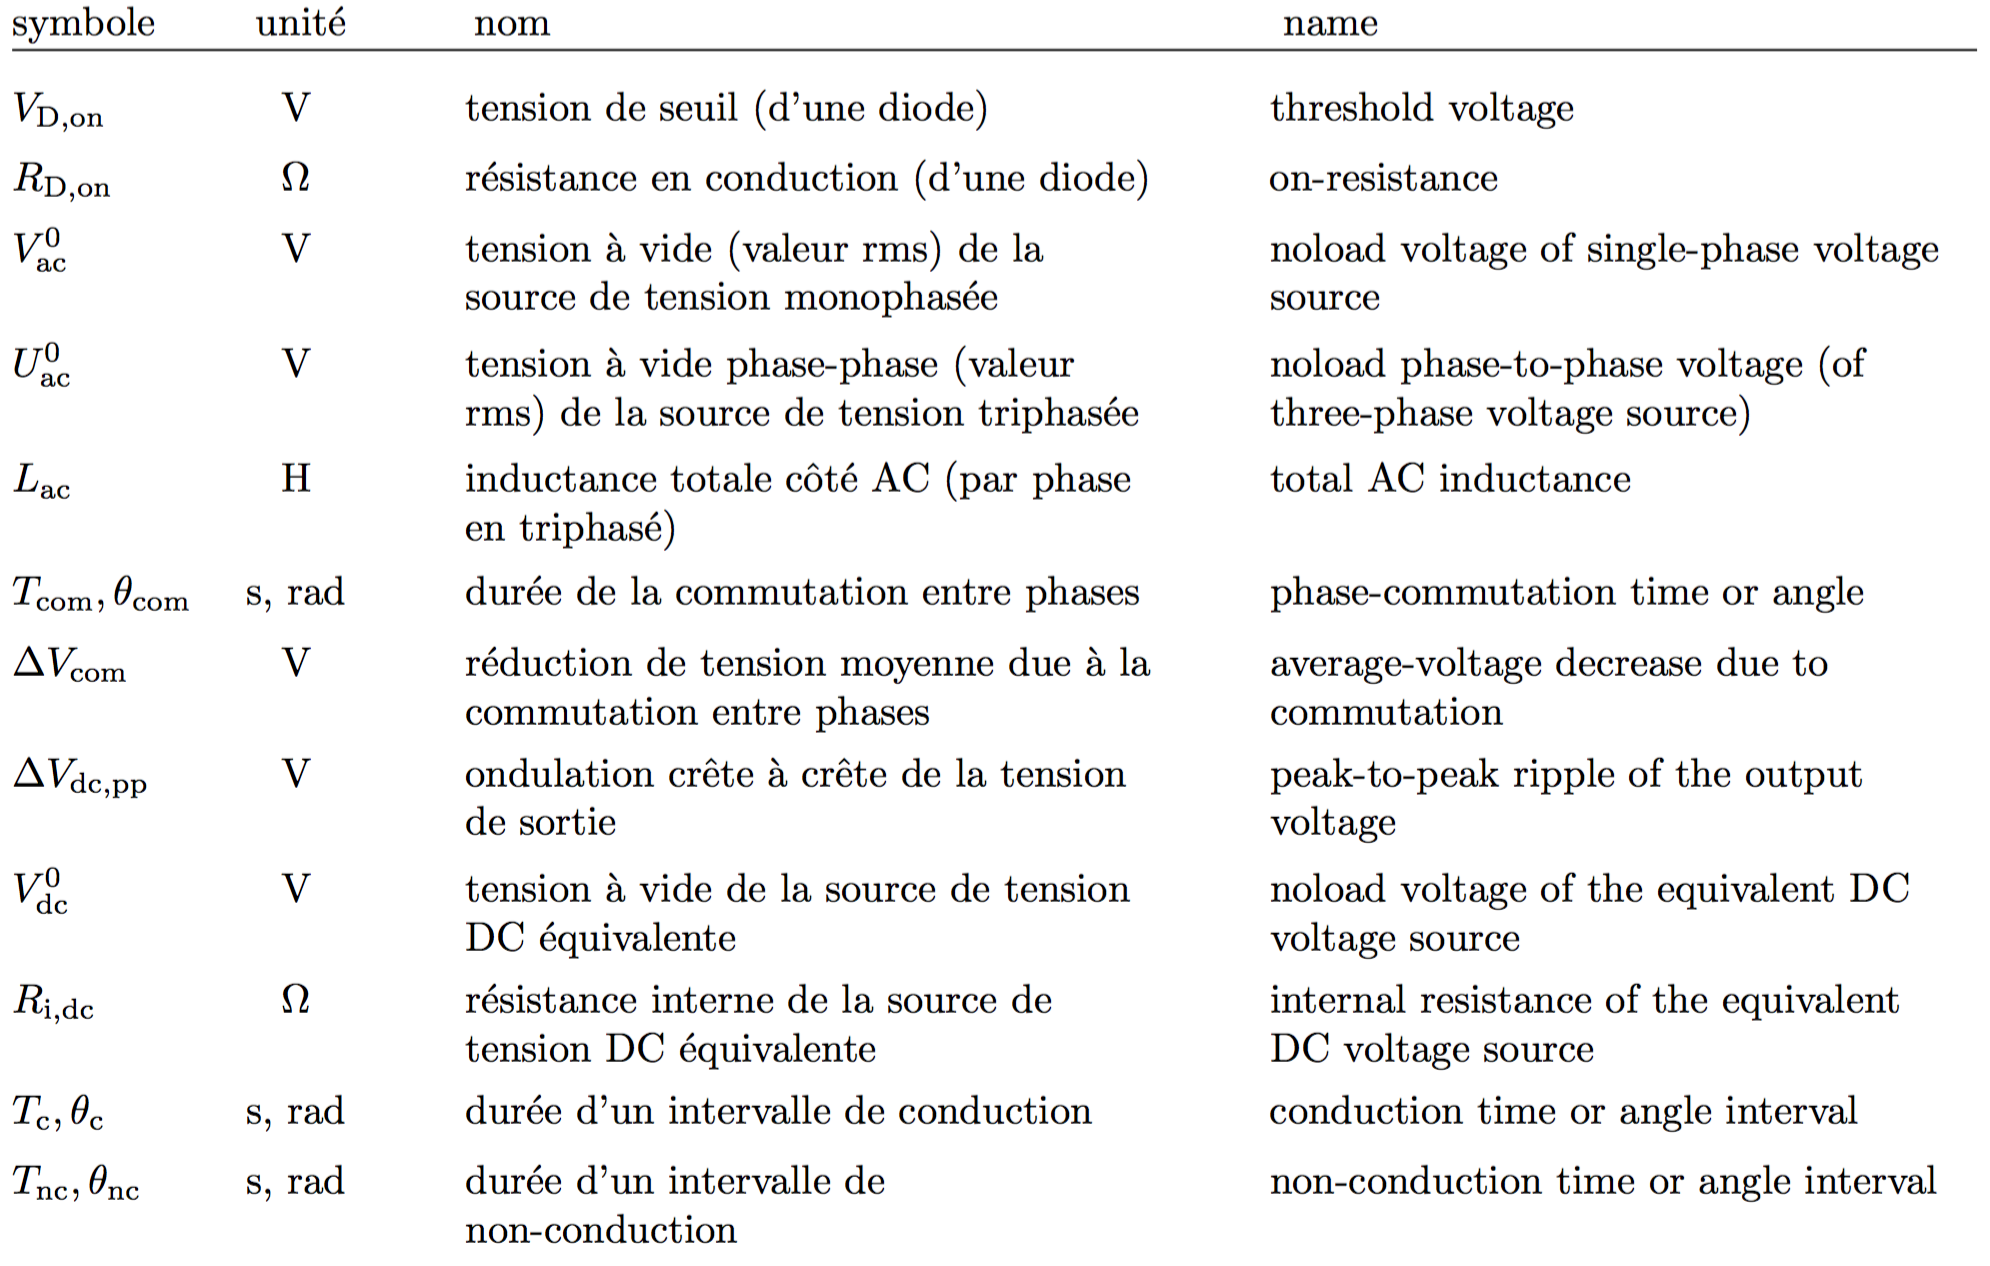
\includegraphics[scale=0.45]{ch2/1}
	\captionof{table}{Liste des symboles.}
	\end{center}
	\newpage
	
	\section{Caractéristique des diodes}
		La figure ci-dessous reprend la représentation réelle à idéalisée de la diode. Elle est \textbf{conductrice} ou passante pour $v_D=v_{AK}$ positive. La tension dépend alors peu du courant $i_D$. 
		
		\begin{center}
		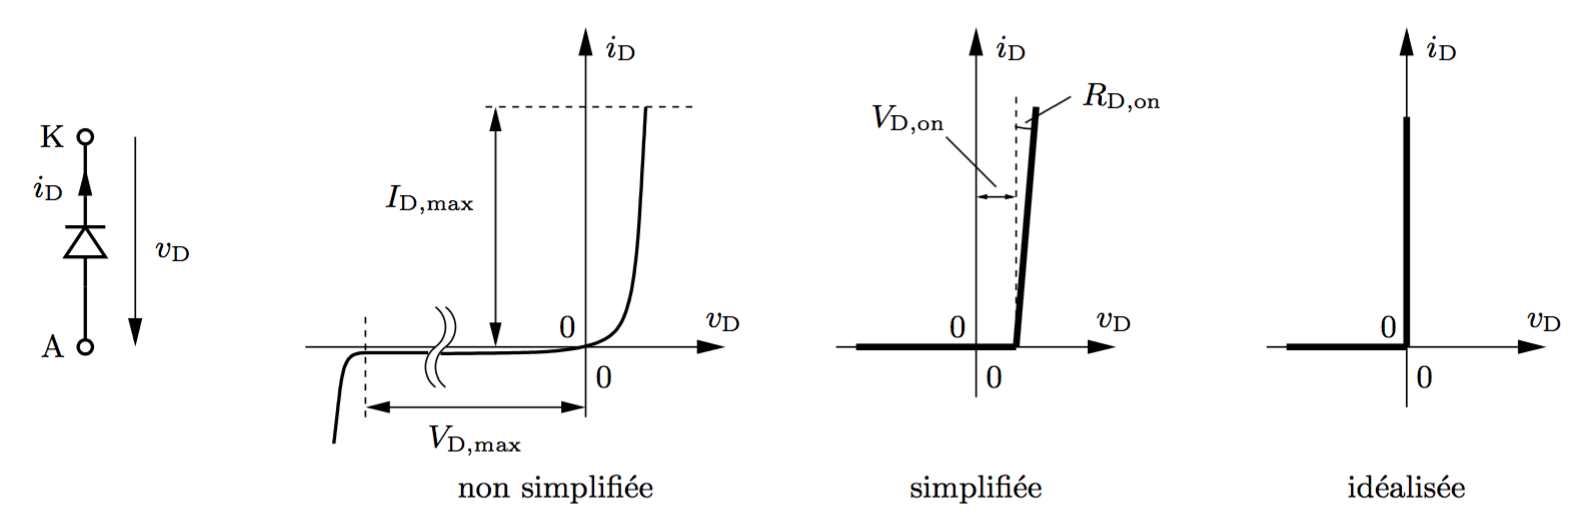
\includegraphics[scale=0.45]{ch2/2}
		\captionof{figure}{}
		\end{center}			
		
		Le courant maximum qu'elle peut supporter, noté $i_{D,max}$ dépend de sa construction, sa taille et du radiateur, refroidisseur sur lequel elle est montée et peut atteindre plusieurs $kA$ pour celles sur le commerce. Pour les diodes de puissance, le transfert de chaleur vers le radiateur est essentiel. De plus elles ont une faible \textbf{inertie thermique} vu leur taille. Pour le modèle simplifié on a en conduction :
		\begin{equation}
			v_D = v_{D,on} + R_{D,on} i_D
		\end{equation}
		où $v_{D,on}$ est appelé \textbf{tension de seuil} et est de l'ordre du volt. Sauf pour les basses tensions (dizaine de volts ou moins), on négligera cette tension $v_D$ car elle influence peu les caractéristiques macroscopique des convertisseurs. On n'oubliera cependant pas qu'il existe une \textbf{perte de conduction} instantanée $P_D(t) = v_D(t)i_D(t)$. \\
	
		Pour ce qui est de l'état \textbf{bloquant} ou \textbf{bloqué}, il se manifeste lorsque $v_D < 0$ et $i_D$ sera négatif mais négligeable. La tension inverse maximum qu'on peut appliquer est noté $v_{D,max}$ et vaut plusieurs $kV$. Les diodes de puissance sont utilisées à des faibles \textbf{fréquences de commutation} (50 ou 60 $Hz$).
	
	\section{Charge inductive générique et circuits redresseurs élémentaires à une ou deux diodes}
		\subsection{Charge RLE générique}
			Pour l'étude des circuits, on considèrera une charge inductive générique RLE. Ces paramètres sont supposés constant c'est à dire que leur variation sur un cycle d'alimentation AC est négligeable. Ceci représente par exemple le circuit d'induit d'une MCC ($E_{dc}\neq 0$) ou son circuit d'excitation ($E_{dc}=0$). L'équation différentielle pour la tension aux bornes de la charge est :
			\begin{equation}
				v_{dc} = E_{dc} + R_{dc}i_{dc} + L_{dc}\frac{di_{dc}}{dt}.
			\end{equation}
			En régime établi et en introduisant la \textbf{tension moyenne} $V_{dc}$ et le \textbf{courant moyen} $I_{dc}$, on a :
			
			\begin{equation}
				V_{dc} = E_{dc} + R_{dc} I_{dc}.
			\end{equation}
			La charge étant alimenté par un redresseur à diode, $i_{dc}$ et $I_{dc}$ ne peuvent pas être négatifs et si $E_{dc}$ est trop élevé, le courant est nul. On a :
			\begin{equation}
				I_{dc} = max\left(\frac{V_{dc} - E_{dc}}{R_{dc}}, 0\right).
			\end{equation}
			
			L'inductance de la charge tend à lisser le courant. C'est d'autant plus le cas que la constante de temps $\tau = L_{dc}/R_{dc}$ est grand par rapport à $T=1/f$ du réseau. Pour les ponts monophasé ou triphasé c'est l'intervalle de temps $T/2$ ou $T/6$ qui importe. Dans le cas d'une MCC, les ondulations de la tension implique une ondulation du courant et donc une ondulation du \textbf{couple électromagnétique}, ce qui est dérangeant. On peut donc adjoindre une inductance extérieur si c'est insuffisant, au détriment de performance dynamique réduits en cas de commande de couple, vitesse ou de position de l'entraînement électrique. 
			
		\subsection{Circuits redresseurs élémentaires avec une diode et une charge R, ER ou EL}
			\subsubsection{Avec charge R}
				La figure ci-dessous représente un circuit avec une source de tension AC de fréquence $f$ idéale raccordée à une diode idéale et une résistance avec $R_{dc}$ constante. Dans ce cas, $i_{ac}(t)=i_{dc}(t)$ à tout instant. La diode n'est passante que lorsque $v_{ac}(t)>0$, avec $v_{dc}(t)=v_{ac}(t)$ et $i_{dc}=v_{ac}(t)/R_{dc}$. La diode est bloquante lorsque $v_D=v_{ac}<0$, avec $v_{dc}=0=i_{dc}$.
				
				\begin{center}
					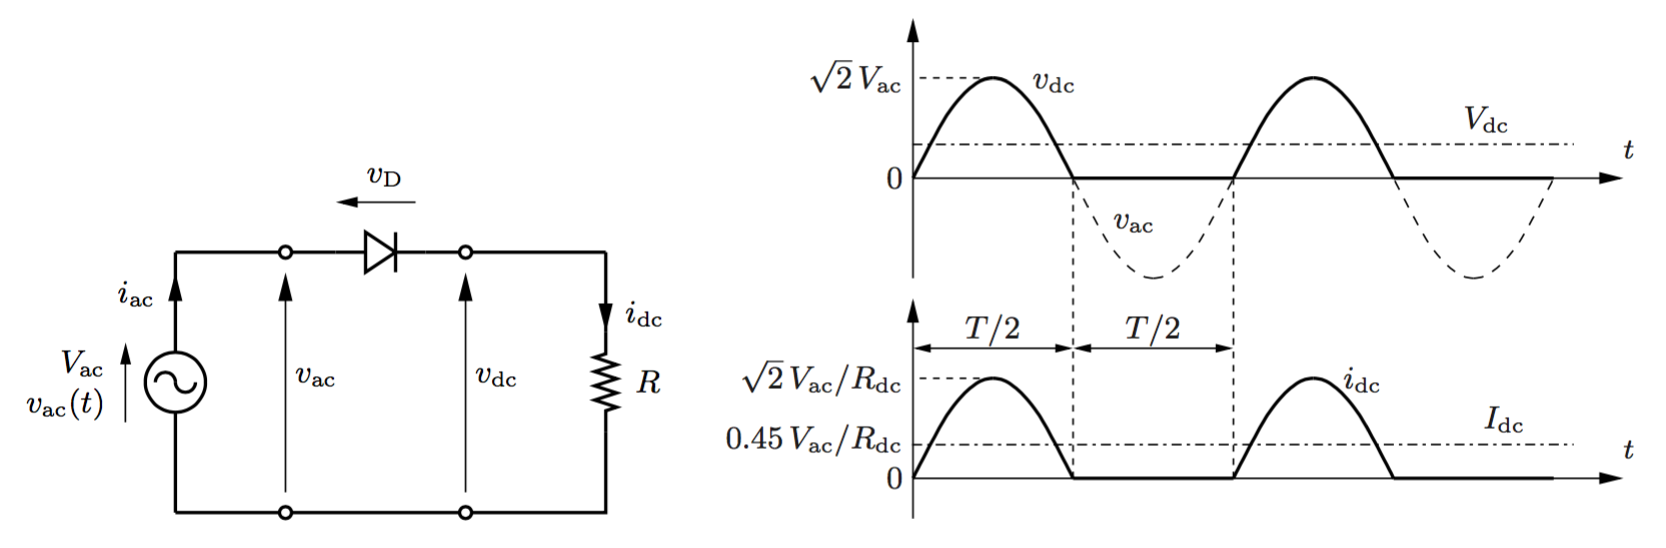
\includegraphics[scale=0.45]{ch2/3}
					\captionof{figure}{}
				\end{center}
				
				On obtient la valeur moyenne de la tension en intégrant sur une demi-période de conduction :
				\begin{equation}
					V_{dc} = \frac{1}{2\pi} \int _0^\pi \sqrt{2}V_{ac}\sin (\omega t) \, d\omega t = \underbrace{\frac{\sqrt{2}}{\pi}}_{0.450} V_{ac}.
					\label{eq:2.5}
				\end{equation}
				
				La tension redressée et le courant $i_{dc}=i_{ac}$ sont fortement ondulés, tous les harmoniques de fréquence $kf$ sont présents (pas de symétrie demi-onde). Le fait qu'un courant continu à moyenne non nul est tiré de la source pose un problème et provient d'un seul chemin $\Rightarrow$ \textbf{redresseur simple voie}. 
				
			\subsubsection{Avec charge ER}
				On a cette fois en plus une source de tension DC dans la charge et on peut voir le montage comme si on chargait une batterie avec résistance interne. 
				
				\begin{center}
				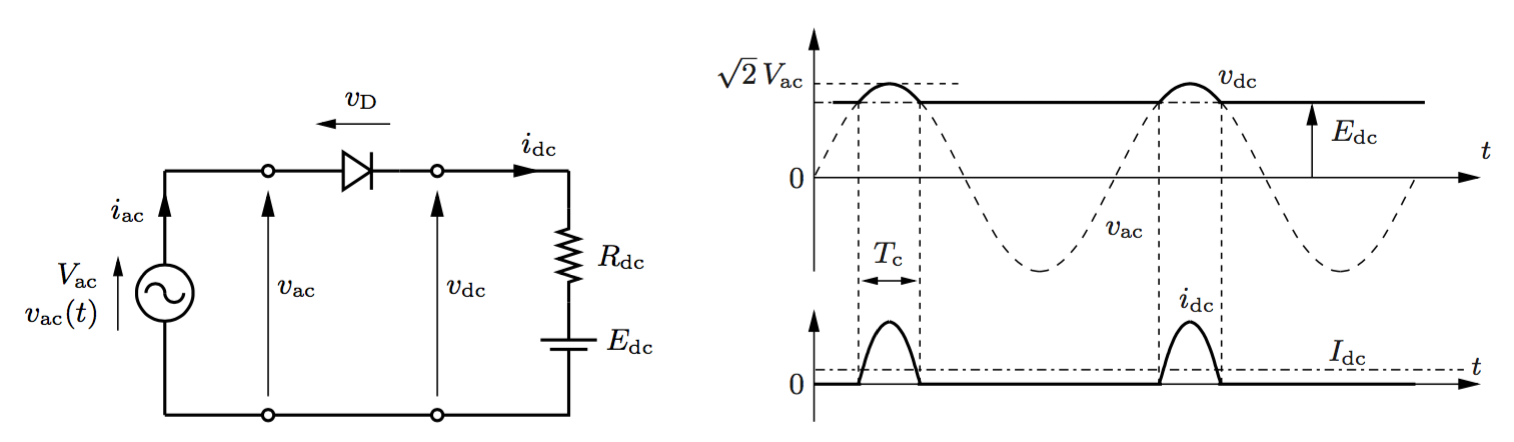
\includegraphics[scale=0.45]{ch2/4}
				\captionof{figure}{}
				\end{center}			 
				
				Dans le cas où la diode est passante, $v_{ac}(t) = v_{dc}(t) = E_{dc} + R_{dc}I_{dc}$, à la condition que $(v_{ac}-E_{dc})/R_{dc}>0$ donc que $v_{ac}>E_{dc}$. Dans le cas d'une diode bloquante, on a $v_{dc} = E_{dc}$. Les grandeurs DC déformées contiennent de nouveau tous les harmoniques de fréquence $kf$ et on a pour les intervalles de conduction de largeur $T_c$ ou $\theta _c = \omega T_c$ : 
				\begin{equation}
					E_{dc} = \hat{V}_{ac} \sin \left(\frac{\pi}{2} - \frac{\theta _c}{2}\right) = \hat{V}_{ac} \cos \frac{\theta _c}{2} \qquad \Rightarrow \qquad \theta _c = 2 \arccos \frac{E_{dc}}{\hat{V}_{ac}}
				\end{equation}
				où on remarque que les intervalles sont d'autant plus court que $E_{dc}$ tend vers $\hat{V}_{ac}$. La tension $V_{dc}$ moyenne s'obtient en intégrant sur $\theta _c$ et les $2\pi - \theta _c$ restant : 
				\begin{equation}
				\begin{aligned}
					\frac{V_{dc}}{\hat{V}_{ac}} &= \frac{1}{2\pi\hat{V}_{ac}} \left[ \int _0 ^{2 \arccos \frac{E_{dc}}{\hat{V}_{ac}}} \hat{V}_{ac} \sin \omega t\,  d\omega t + \int _{2 \arccos \frac{E_{dc}}{\hat{V}_{ac}}} ^{2\pi} E_{dc} \, d\omega t \right]\\
								&= \frac{1}{\pi} \sqrt{1 - \left(\frac{E_{dc}}{\hat{V}_{ac}}\right)^2} + \left(1- \frac{1}{\pi} \arccos \frac{E_{dc}}{\hat{V}_{ac}} \right)
				\end{aligned}
				\end{equation}
				
	\subsection{Circuit avec une diode redresseuse et une diode de roue libre - empiètement}
		\begin{wrapfigure}[11]{l}{5.5cm}
		\vspace{-5mm}
		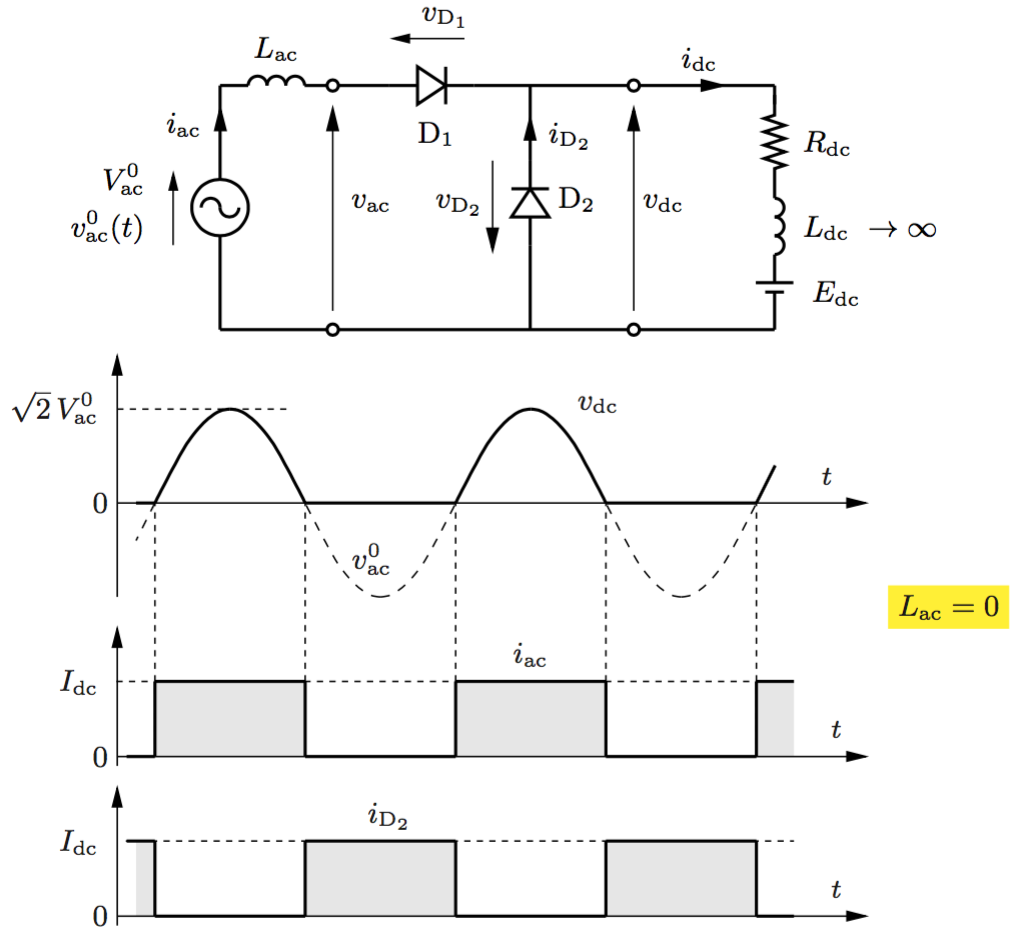
\includegraphics[scale=0.3]{ch2/5}
		\captionof{figure}{}
		\end{wrapfigure}
		Sur la figure ci-contre sont représenté deux diodes D1 et D2, la 1ère laissant conduire la source de tension AC et la 2è dites de roue libre étant un chemin supplémentaire pour le courant dans la charge. La source AC est modélisé par son équivalent à vide $v_{ac}^0(t)$ et une inductance interne $L_{ac}$. Prenons d'abord le cas où $L_{dc} \rightarrow \infty$, lissant parfaitement le courant $i_{dc} = I_{dc}$. Il s'agit toujours d'un redresseur simple voie car le courant n'est pas alternatif. \\\\\\
		
		\subsubsection{Avec source de tension AC idéale et charge infiniment inductive}
			Supposons d'abord que $L_{ac} = 0$, on a alors avec $L_{dc} = \infty$ : 
			\begin{equation}
				I_{dc} = i_{ac} + i_{D2}.
			\end{equation}
			
			On peut très bien faire l'expérience de la pensée qui conclue que le courant de la charge sera fourni par la source AC lors des alternances positives et circulera dans D2 lors des alternances négatives. La commutation entre les 2 diodes est instantannée. La valeur de tension moyenne se calcule comme \eqref{eq:2.5}. Lors des alternances négatives, la D2 étant passante, $-v_{D2} = v_{dc} = 0$. Toute la tension se retrouve alors sur D1.  
			
		\subsubsection{Avec source de tension AC non idéale et charge infiniment inductive}
			\begin{wrapfigure}[10]{l}{5.5cm}
			\vspace{-5mm}
			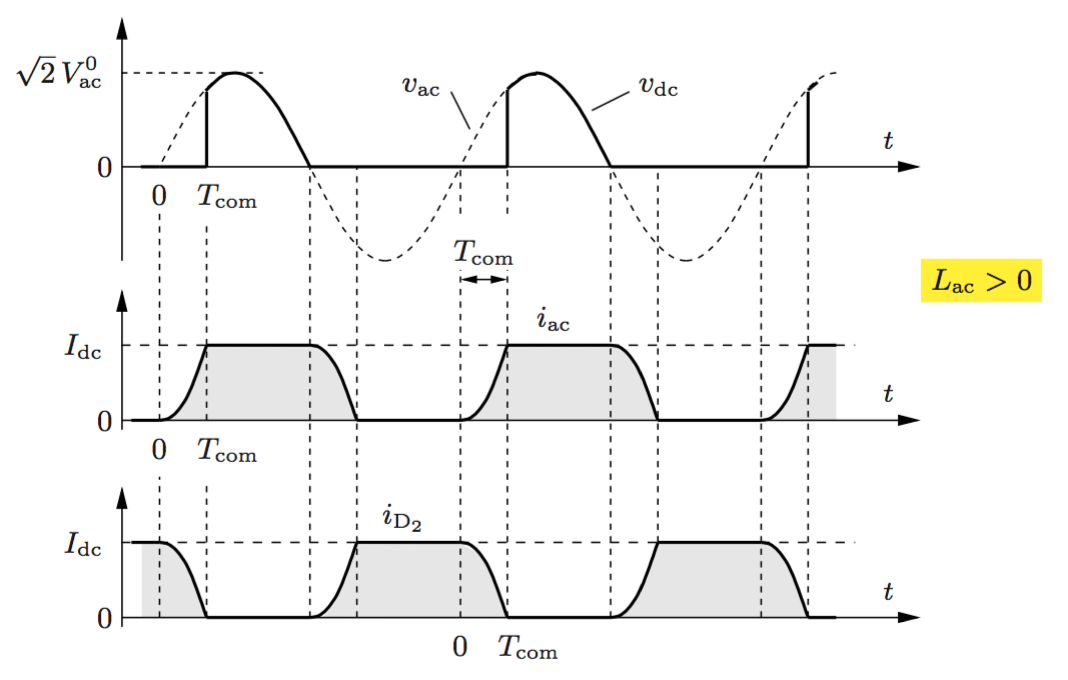
\includegraphics[scale=0.3]{ch2/6}
			\captionof{figure}{}
			\end{wrapfigure}
			Dans ce cas, $L_{ac}$ empêche les variations instantanées du courant lors des commutations. L'intervalle de temps est désigné par $T_{com}$, pendant lequel les 2 diodes conduisent en même temps, on parle d'\textbf{empiètement} ou de \textbf{recouvrement}. L'équation de la maille de gauche nous permet d'écrire avec les 2 diodes conductrices : 
			\begin{equation}
				v_{ac}^0 (t) = \sqrt{2} V_{ac}^0 \sin \omega t = Li_{ac}\frac{di_{ac}(t)}{dt}.
				\label{eq:2.9}
			\end{equation}
			On a comme précédemment $v_{dc}(t) = - v_{D2}(t) = 0$. Intéressons-nous dans un premier temps à la commutation de D2 vers D1 (0 à $T_{com}$). En intégrant \eqref{eq:2.9} comme suit : 
			\begin{equation}
			\begin{aligned}
				&\int _0 ^{\omega T_{com}} \sqrt{2} V_{ac}^0 \sin \omega t \, d\omega t = \int _0 ^{I_{dc}} Li_{ac}\, di_{ac} \\
				\Leftrightarrow \quad &\sqrt{2} V_{ac}^0 (1- \cos \omega T_{com}) = \omega L_{ac} I_{dc}\\
				\Leftrightarrow \quad &\theta _{com} = \omega T_{com} = \arccos \left( 1 - \frac{\omega L_{ac}}{\sqrt{2} V_{ac}^0}I_{dc} \right)
				\end{aligned}
			\end{equation}			 
			On remarque ici que la durée de la commutation est d'autant plus grande que le courant et l'inductance sont grands. Le retard sur la hausse de tension induit une baisse de la valeur moyenne de la tension de sortie désignée par $\Delta V_{com}$ : 			
			\begin{equation}
				\Delta V_{com} = \frac{1}{2\pi} \int _0 ^{\omega T_{com}} v_{ac}^0(t) \, d\omega t = \frac{1}{2\pi} \int _0 ^{\omega T_{com}} \omega L_{ac}\frac{di_{ac}}{dt} \, dt = \frac{\omega L_{ac}}{2\pi} I_{dc}.
 			\end{equation}
 			On voit que les même conclusion sont valables pour la chute de tension moyenne. 